\section{Placement}

The placement of the I/O routers in a large 3D torus can have an enormous impact
on the traffic patterns and congestion characteristics present in the system.
This is important for maximizing I/O performance as well as minimizing the
interaction between application communication and I/O. Building on the lessons
learned from OLCF's Spider~I implementation of fine-grained routing in 2008, an
improved method for placing LNET routers on Titan was developed and implemented
for Spider~II.

\begin{figure*}[t]
  \begin{center}
    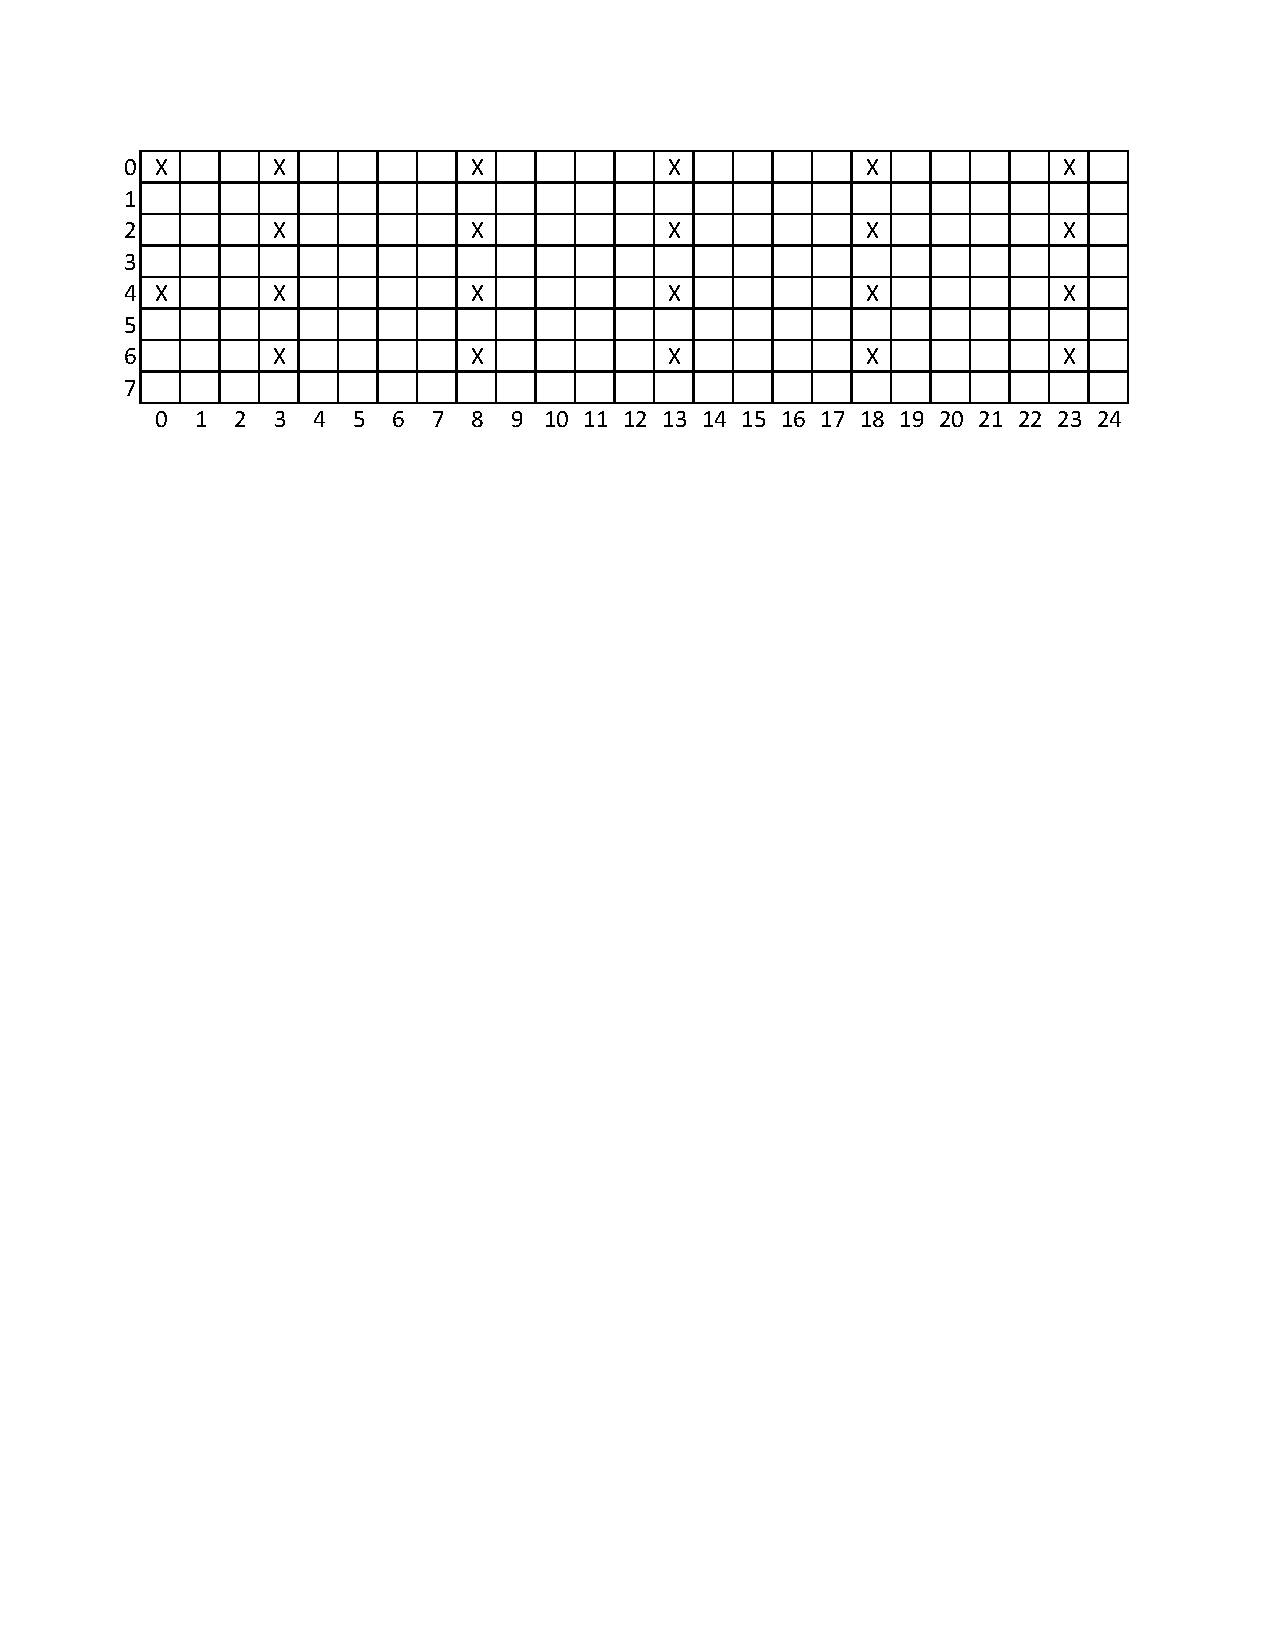
\includegraphics{figures/jaguarplacement}
    \caption{Jaguar Layout}\label{fig:jaglayout}
  \end{center}
\end{figure*}
\begin{figure*}[t]
  \begin{center}
    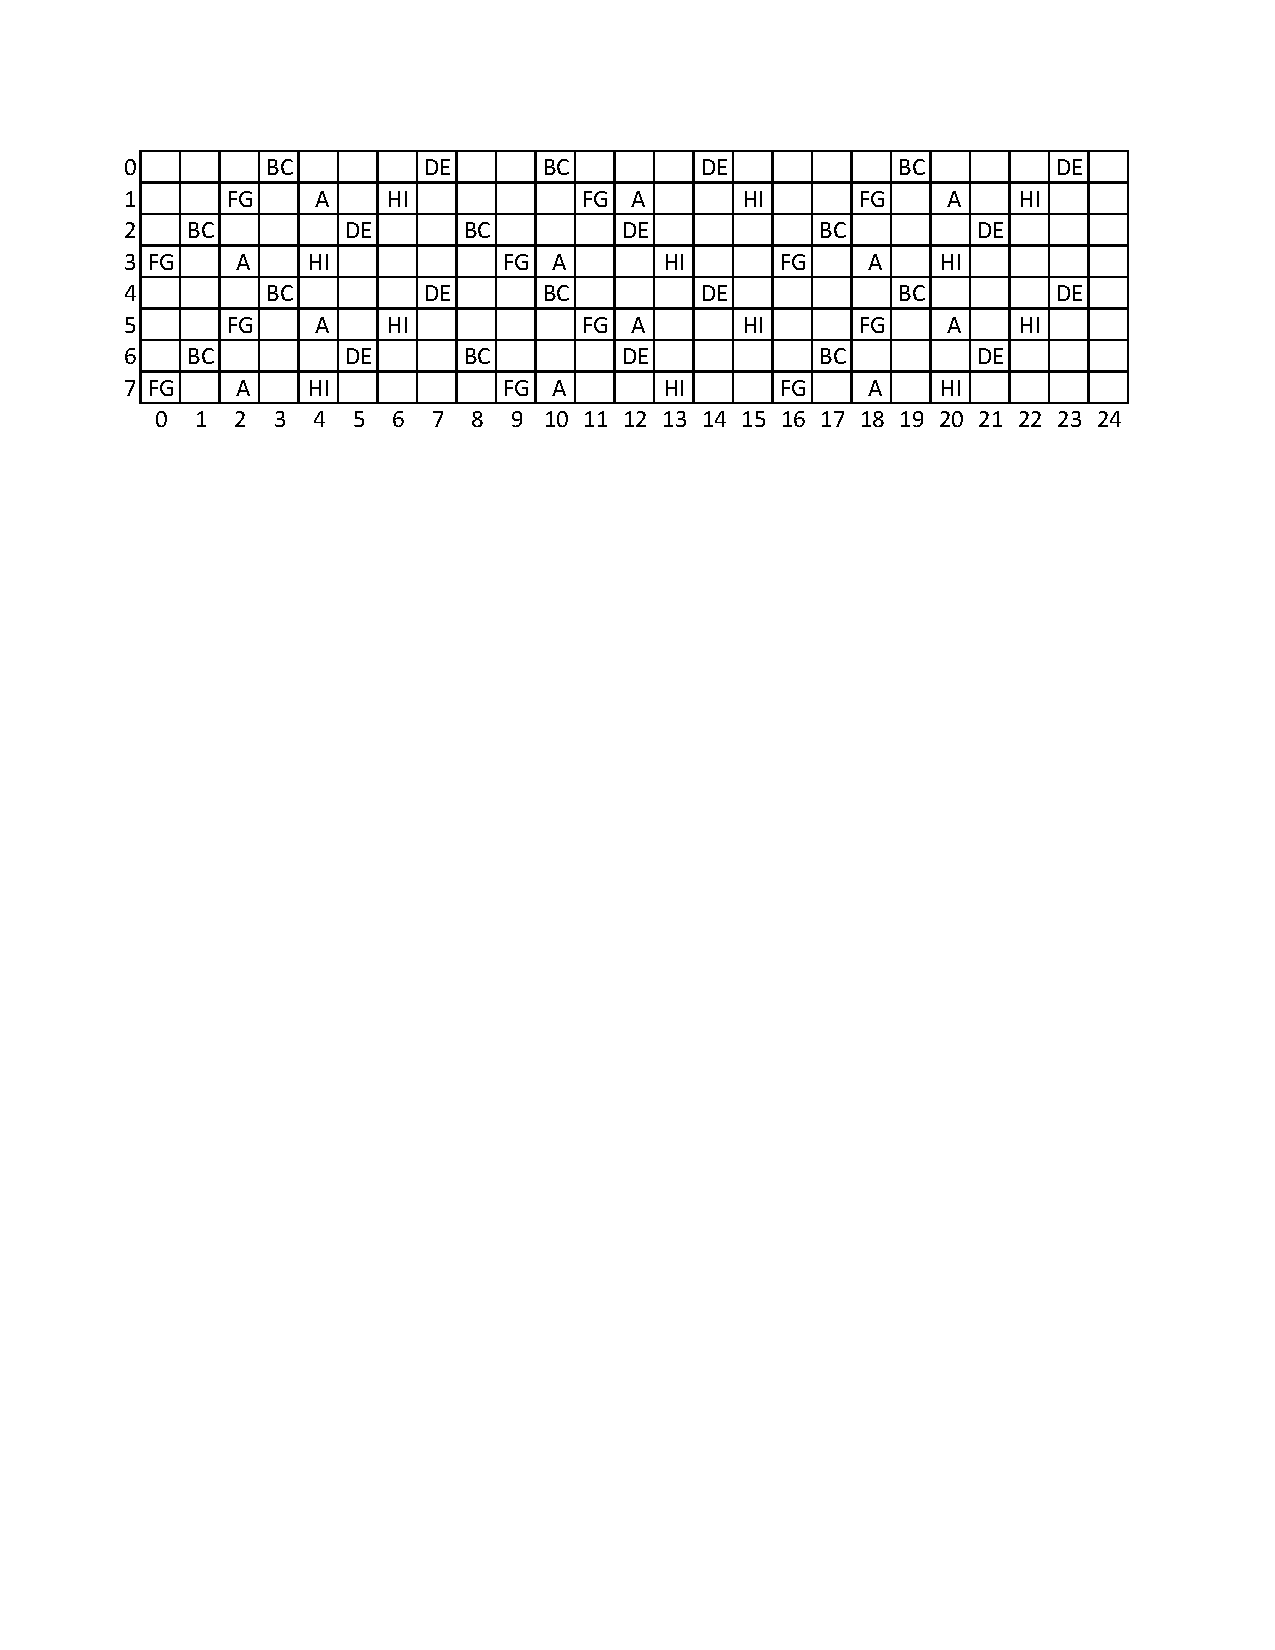
\includegraphics{figures/titanplacement}
    \caption{Titan Layout}\label{fig:titanlayout}
  \end{center}
\end{figure*}

\subsection{Topological Concerns}
\label{sec:topo}

The router placement layout used for Spider~I was designed to distribute the
routers topologically through the machine while also minimizing the number of
cabinets that contained routers (see Figure \ref{fig:jaglayout}). This resulted
in a very regular I/O pattern that was prone to congestion if I/O traffic was
not properly kept localized.

Details about Gemini's architecture and performance characteristics are
available in a paper titled ``Understanding the Impact of Interconnect Failures
on System Operation'' \cite{interconnect} presented at CUG 2013.  Jaguar's
upgrade from Cray's SeaStar interconnect to Gemini significantly changed the
network's characteristics.  Each Gemini supports two nodes, which effectively
halved the Y-dimension length.  Additionally, Y-dimension connections are
comprised of only half the links of X- and Z-dimension connections.  Thus, I/O
traffic should be limited in the Y-dimension due to its reduced relative
bandwidth.  This suggests that routing zones should be ``flattened'' into
``rectangular prisms'' instead of the more traditional cubic zones.

Since Gemini uses dimension-ordered-routing, I/O tends to converge to a single
path as it nears the destination.  Thus, it is important to avoid putting
routers in the same plane.  This can help avoid congestion, but many-to-one
communication patterns in a 3D torus will always suffer from some amount of
congestion.

Minimizing the hop count between clients and routers is essential for providing
high-bandwidth communications with the storage servers.  While Gemini routing
arbitration is locally fair, it is globally unfair.  Packet age and hop-count
are not taken into account when the router selects the next packet to forward.
Figure \ref{fig:geombw} shows an example of this issue.

\begin{figure}[h]
  \centering
    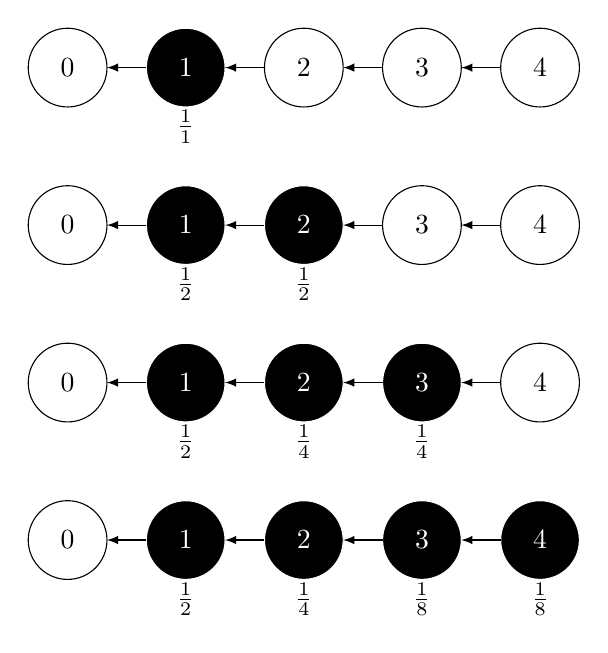
\begin{tikzpicture}
    \def \phase {1}
    \node[draw, circle, minimum height=1cm] at (0,-\phase){$0$};
    \node[draw, circle, minimum height=1cm, color=white, fill=black] at (1.5,-\phase){$1$};
    \node[draw, circle, minimum height=1cm] at (3,-\phase){$2$};
    \node[draw, circle, minimum height=1cm] at (4.5,-\phase){$3$};
    \node[draw, circle, minimum height=1cm] at (6,-\phase){$4$};
    \draw[->, >=latex] (1.0,-\phase) to (0.5,-\phase);
    \draw[->, >=latex] (2.5,-\phase) to (2.0,-\phase);
    \draw[->, >=latex] (4.0,-\phase) to (3.5,-\phase);
    \draw[->, >=latex] (5.5,-\phase) to (5.0,-\phase);
    \node[draw=none] at (1.5,-1.75) {$\frac{1}{1}$};

    \def \phase {3}
    \node[draw, circle, minimum height=1cm] at (0,-\phase){$0$};
    \node[draw, circle, minimum height=1cm, color=white, fill=black] at (1.5,-\phase){$1$};
    \node[draw, circle, minimum height=1cm, color=white, fill=black] at (3,-\phase){$2$};
    \node[draw, circle, minimum height=1cm] at (4.5,-\phase){$3$};
    \node[draw, circle, minimum height=1cm] at (6,-\phase){$4$};
    \draw[->, >=latex] (1.0,-\phase) to (0.5,-\phase);
    \draw[->, >=latex] (2.5,-\phase) to (2.0,-\phase);
    \draw[->, >=latex] (4.0,-\phase) to (3.5,-\phase);
    \draw[->, >=latex] (5.5,-\phase) to (5.0,-\phase);
    \node[draw=none] at (1.5,-3.75) {$\frac{1}{2}$};
    \node[draw=none] at (3,-3.75) {$\frac{1}{2}$};

    \def \phase {5}
    \node[draw, circle, minimum height=1cm] at (0,-\phase){$0$};
    \node[draw, circle, minimum height=1cm, color=white, fill=black] at (1.5,-\phase){$1$};
    \node[draw, circle, minimum height=1cm, color=white, fill=black] at (3,-\phase){$2$};
    \node[draw, circle, minimum height=1cm, color=white, fill=black] at (4.5,-\phase){$3$};
    \node[draw, circle, minimum height=1cm] at (6,-\phase){$4$};
    \draw[->, >=latex] (1.0,-\phase) to (0.5,-\phase);
    \draw[->, >=latex] (2.5,-\phase) to (2.0,-\phase);
    \draw[->, >=latex] (4.0,-\phase) to (3.5,-\phase);
    \draw[->, >=latex] (5.5,-\phase) to (5.0,-\phase);
    \node[draw=none] at (1.5,-5.75) {$\frac{1}{2}$};
    \node[draw=none] at (3,-5.75) {$\frac{1}{4}$};
    \node[draw=none] at (4.5,-5.75) {$\frac{1}{4}$};

    \def \phase {7}
    \node[draw, circle, minimum height=1cm] at (0,-\phase){$0$};
    \node[draw, circle, minimum height=1cm, color=white, fill=black] at (1.5,-\phase){$1$};
    \node[draw, circle, minimum height=1cm, color=white, fill=black] at (3,-\phase){$2$};
    \node[draw, circle, minimum height=1cm, color=white, fill=black] at (4.5,-\phase){$3$};
    \node[draw, circle, minimum height=1cm, color=white, fill=black] at (6,-\phase){$4$};
    \draw[->, >=latex] (1.0,-\phase) to (0.5,-\phase);
    \draw[->, >=latex] (2.5,-\phase) to (2.0,-\phase);
    \draw[->, >=latex] (4.0,-\phase) to (3.5,-\phase);
    \draw[->, >=latex] (5.5,-\phase) to (5.0,-\phase);
    \node[draw=none] at (1.5,-7.75) {$\frac{1}{2}$};
    \node[draw=none] at (3,-7.75) {$\frac{1}{4}$};
    \node[draw=none] at (4.5,-7.75) {$\frac{1}{8}$};
    \node[draw=none] at (6,-7.75) {$\frac{1}{8}$};
  \end{tikzpicture}


  \caption{Geometric Bandwidth Reductions}\label{fig:geombw}
\end{figure}

Node 0 can be considered an I/O router while the others are acting as clients
attempting to send data to the router.  When only node 0 is communicating, it
is able to achieve 100\% of the bandwidth across the link.  Once node 2 starts
communicating, the router attached to node 1 accepts half the bandwidth from
node 1 and half from node 2.  Effectively, the bandwidth is shared between the
nodes.  When node 3 begins communicating, the router attached to node 2 fairly
arbitrates traffic between nodes 2 and 3.  Since that router only has half of
the global bandwith, nodes 2 and 3 each only get one quarter of the total
bandwith to the router.  When node 4 begins communicating, the problem becomes
even more obvious.  The router attached to node 3 fairly arbitrates traffic
between nodes 3 and 4, but it can only grant one eighth of the total bandwidth
to each.

As these chains get longer and longer, the bandwidth available to the ``last''
node can become abysmal.

\subsection{Physical Constraints}


The following physical constraints and goals were kept in mind while
determining an optimal placement algorithm:

\begin{description}
  \item[Topological Concerns] \hfill \\
    Routers must be placed to optimize for the topological concerns mentioned
    in Section \ref{sec:topo}.
  \item[Minimize Cabinet Count] \hfill \\
    Each cabinet that contains a router module requires a hole to be drilled in
    the floor to accomodate the cables.
  \item[Cable Length] \hfill \\
    Shorter cables are cheaper and easier to manage in the data center.
  \item[Partitionability] \hfill \\
    Occasionally, Titan's 3D torus must be partitioned to facilitate extended
    maintenance activites or testing.  During this situation, it is important to
    ensure full routability to boot from both ``ends'' of the machine.  A boot
    node is located in physical columns 0 and 24 (topological columns 0 and 13).
    Thus, routers should be located in a way that minimizes the number of
    columns required to access the entire file system.
\end{description}

\subsection{Implementation}

In the Cray~XK architecture, each service module contains four service nodes.
Since each service module displaces a compute module, it is important to
utilize each node.  Ideally, the LNET routers would exist on the same module as
less bandwidth-intensive nodes (such as a login nodes).  This is unfortunately
impossible due to the sheer number of routers required to achieve sufficient
bandwidth.

Having 4 routers on a module matches nicely with the 4 rows of Spider~II.  The
nodes on a given module will connect to a switch in each of the 4 rows of
Spider~II.  There is a ``swizzle'' to spread Gemini load.

As part of the Spider~II upgrade, the number of LNET routers on Titan was
doubled to 440 nodes and each router was equipped with an IB FDR HCA with 16
PCI-E lanes running at Gen-2.

% vim:textwidth=80:
